% =============================================================================
% PyCore CALL FSM — systems documentation for the research paper
% =============================================================================
% Build (from this directory):
%   pdflatex call_fsm.tex && pdflatex call_fsm.tex
% Requires: article, tikz, booktabs, hyperref, listings, geometry, microtype
% =============================================================================
\documentclass[11pt,a4paper]{article}

\usepackage[margin=1in]{geometry}
\usepackage{microtype}
\usepackage{booktabs}
\usepackage{tabularx}
\usepackage{graphicx}
\usepackage{xcolor}
\usepackage{hyperref}
\usepackage{listings}
\usepackage{amsmath}
\usepackage{amssymb}
\usepackage{enumitem}
\usepackage{tikz}
\usetikzlibrary{arrows.meta,automata,positioning,fit,calc,shapes.geometric,shapes.multipart}

\hypersetup{
  colorlinks=true,
  linkcolor=black,
  urlcolor=blue!50!black,
  citecolor=black
}

\lstdefinestyle{py}{
  language=Python,
  basicstyle=\ttfamily\footnotesize,
  keywordstyle=\bfseries,
  commentstyle=\itshape\color{gray!60!black},
  showstringspaces=false,
  breaklines=true,
  frame=single,
  rulecolor=\color{black!20},
  columns=fullflexible
}
\lstdefinestyle{sv}{
  language=C,
  basicstyle=\ttfamily\footnotesize,
  keywordstyle=\bfseries,
  commentstyle=\itshape\color{gray!60!black},
  showstringspaces=false,
  breaklines=true,
  frame=single,
  rulecolor=\color{black!20},
  columns=fullflexible,
  morekeywords={logic,localparam,unique,case,endcase,begin,end,always_ff,always_comb}
}
\lstset{style=py}

\title{The PyCore CALL Finite-State Machine\\
\large Shared argument binding for CPython~3.14 bytecode on a research CPU}
\author{PyCore systems notes\\
\texttt{docs/paper/systems/call\_fsm.tex}}
\date{August 2026}

\begin{document}
\maketitle

\begin{abstract}
PyCore executes a CPython~3.14 bytecode subset in hardware.
Function invocation is one of the most semantics-dense paths in that subset:
free functions, bound methods, keyword calls, starred calls, defaults,
positional-only parameters, \texttt{*args}, and \texttt{**kwargs} must all
agree with CPython before higher-level components can rely on ordinary Python
call shapes.
This note documents the \texttt{S\_CALL} finite-state machine and its
\emph{shared binder}---the hardware path that maps caller stack arguments onto
callee locals.
We describe phase structure, call modes, stack layouts, binder micro-sequences,
worked examples, design tradeoffs, and remaining limits.
Primary RTL sources are \texttt{pycore/rtl/pycore\_call\_fsm.svh} and
\texttt{pycore/rtl/pycore\_core.sv}.
\end{abstract}

\tableofcontents
\newpage

% -----------------------------------------------------------------------------
\section{Motivation and scope}
% -----------------------------------------------------------------------------

PyCore's ISA is not a conventional RISC; it is a filtered CPython bytecode.
That choice makes \emph{call} a first-class microarchitectural concern rather
than a compiler ABI detail.
CPython~3.14 emits three related opcodes for ordinary calls:

\begin{center}
\begin{tabular}{@{}llp{0.52\textwidth}@{}}
\toprule
Opcode & Hex & Role \\
\midrule
\texttt{CALL} & 52 & Positional arguments only \\
\texttt{CALL\_KW} & 55 & Mixed positional + keyword (names tuple at TOS) \\
\texttt{CALL\_FUNCTION\_EX} & 04 & \texttt{*args} / \texttt{**kwargs} expand \\
\bottomrule
\end{tabular}
\end{center}

A fourth opcode, \texttt{DICT\_MERGE}, often precedes \texttt{CALL\_FUNCTION\_EX}
when the caller writes \texttt{f(*a, **d)}.
PyCore implements merge separately; this document focuses on the CALL FSM that
consumes the resulting stack shape.

\paragraph{Why a dedicated FSM.}
Argument binding is multi-cycle: it reads code-object metadata from dmem,
probes name tuples and default containers, may allocate an \texttt{*args} tuple
or a \texttt{**kwargs} dict, then pushes a hardware frame.
Folding that work into a single ``execute'' beat is neither faithful to CPython
nor practical under PyCore's memory ports.
The FSM therefore sits as core state \texttt{S\_CALL}, with an internal phase
register and a nested binder sub-state machine.

\paragraph{Scope of this note.}
We cover user \texttt{CODE\_OBJECT} callees (the interim model where a function
\emph{is} a code-object handle), method-form calls, bound-method unwrap, type
instantiation entry, and the on-core builtin fast path at a high level.
We do not re-derive excore grow handlers or the full object model; those are
sibling systems notes.

% -----------------------------------------------------------------------------
\section{Architectural placement}
% -----------------------------------------------------------------------------

Figure~\ref{fig:placement} places CALL in the core control loop.
Decode recognizes \texttt{CALL} / \texttt{CALL\_KW} / \texttt{CALL\_FUNCTION\_EX}
and enters \texttt{S\_CALL}.
On success the FSM ends in \texttt{CALL\_PHASE\_DONE}, which redirects fetch to
the callee entry and leaves the value stack ready for the callee body.
On failure it raises a trap---most often \texttt{PY\_TRAP\_CALL\_FILTER} (code~6),
PyCore's fatal stand-in for CPython \texttt{TypeError} on bad call shapes.

\begin{figure}[ht]
\centering
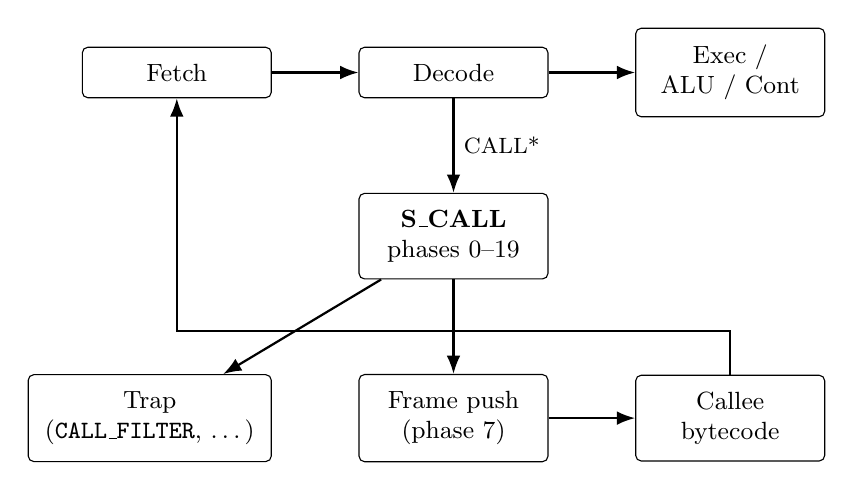
\begin{tikzpicture}[
  font=\small,
  box/.style={draw, rounded corners=2pt, align=center, inner sep=6pt, minimum width=2.4cm},
  arr/.style={-{Latex}, thick}
]
  \node[box] (fetch) {Fetch};
  \node[box, right=1.1cm of fetch] (dec) {Decode};
  \node[box, right=1.1cm of dec] (exec) {Exec /\\ALU / Cont};
  \node[box, below=1.2cm of dec] (call) {\textbf{S\_CALL}\\phases 0--19};
  \node[box, below=1.2cm of call] (frame) {Frame push\\(phase 7)};
  \node[box, left=1.1cm of frame] (trap) {Trap\\(\texttt{CALL\_FILTER}, \ldots)};
  \node[box, right=1.1cm of frame] (run) {Callee\\bytecode};

  \draw[arr] (fetch) -- (dec);
  \draw[arr] (dec) -- (exec);
  \draw[arr] (dec) -- node[right, font=\footnotesize]{CALL*} (call);
  \draw[arr] (call) -- (frame);
  \draw[arr] (call) -- (trap);
  \draw[arr] (frame) -- (run);
  \draw[arr] (run.north) |- ++(0,0.55) -| (fetch.south);
\end{tikzpicture}
\caption{CALL in the PyCore control hierarchy.
\texttt{S\_CALL} owns argument normalization and binding; frame push is a
distinct phase that consumes the binder's effective argc.}
\label{fig:placement}
\end{figure}

% -----------------------------------------------------------------------------
\section{Call modes}
% -----------------------------------------------------------------------------

\texttt{call\_mode\_r} records how the caller presented arguments:

\begin{center}
\begin{tabular}{@{}clp{0.62\textwidth}@{}}
\toprule
Mode & Value & Meaning \\
\midrule
\texttt{CALL\_MODE\_POS} & 0 & Plain \texttt{CALL}; oparg $=$ positional count \\
\texttt{CALL\_MODE\_KW} & 1 & \texttt{CALL\_KW}; TOS is names \texttt{TUPLE} \\
\texttt{CALL\_MODE\_EX} & 2 & \texttt{CALL\_FUNCTION\_EX} expand in progress \\
\texttt{CALL\_MODE\_EX\_KW} & 3 & EX path with a kwargs \texttt{MUT\_DICT} \\
\bottomrule
\end{tabular}
\end{center}

\texttt{CALL\_FUNCTION\_EX} always begins in mode \texttt{EX}.
After the kwargs sentinel/dict and args list/tuple are classified, the FSM either
joins the positional path (\texttt{POS}) or the keyword binder (\texttt{EX\_KW}).
That join is intentional: once starred arguments are expanded onto the stack,
binding is the same problem as \texttt{CALL}/\texttt{CALL\_KW}.

% -----------------------------------------------------------------------------
\section{Phase map}
% -----------------------------------------------------------------------------

Figure~\ref{fig:phases} is the top-level phase automaton.
Phases~0--7 are the common \texttt{CODE\_OBJECT} path.
Phases~8--13 handle non-code callables.
Phases~16--19 are entry preludes for keyword and starred forms.

\begin{figure}[ht]
\centering
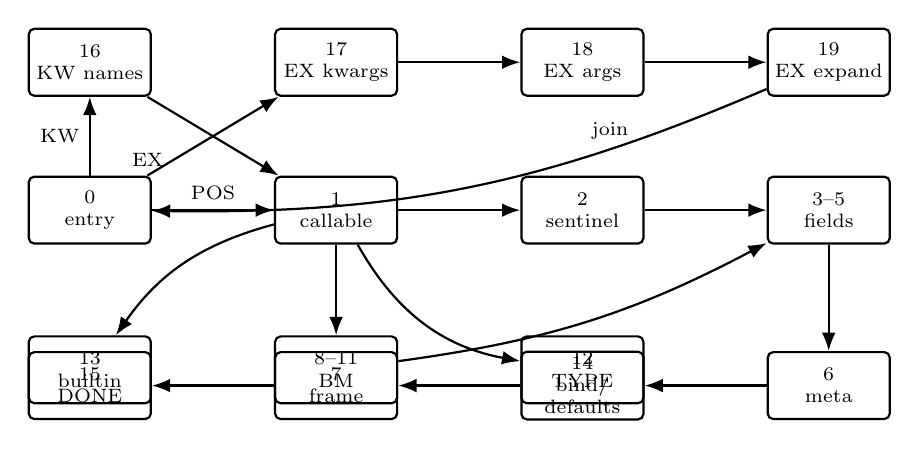
\begin{tikzpicture}[
  font=\scriptsize,
  auto,
  thick,
  node distance=1.35cm and 1.55cm,
  state/.style={draw, rounded corners=2pt, align=center, minimum width=1.55cm, minimum height=0.85cm, inner sep=2pt},
  every edge/.style={draw, -{Latex}}
]
  \node[state] (p0) {0\\entry};
  \node[state, right=of p0] (p1) {1\\callable};
  \node[state, right=of p1] (p2) {2\\sentinel};
  \node[state, right=of p2] (p3) {3--5\\fields};
  \node[state, below=of p3] (p6) {6\\meta};
  \node[state, left=of p6] (p14) {14\\bind/\\defaults};
  \node[state, left=of p14] (p7) {7\\frame};
  \node[state, left=of p7] (done) {15\\DONE};

  \node[state, above=1.0cm of p0] (kw) {16\\KW names};
  \node[state, above=1.0cm of p1] (exk) {17\\EX kwargs};
  \node[state, above=1.0cm of p2] (exa) {18\\EX args};
  \node[state, above=1.0cm of p3] (exe) {19\\EX expand};

  \node[state, below=1.15cm of p1] (obj) {8--11\\BM};
  \node[state, below=1.15cm of p2] (ty) {12\\TYPE};
  \node[state, below=1.15cm of p0] (bi) {13\\builtin};

  \path (p0) edge node[above]{POS} (p1);
  \path (p0) edge node[left]{KW} (kw);
  \path (p0) edge node[left, pos=0.2]{EX} (exk);
  \path (kw) edge (p1);
  \path (exk) edge (exa);
  \path (exa) edge (exe);
  \path (exe) edge[bend left=12] node[above, pos=0.25]{join} (p0);
  \path (p1) edge (p2);
  \path (p1) edge (obj);
  \path (obj) edge[bend right=10] (p3);
  \path (p2) edge (p3);
  \path (p3) edge (p6);
  \path (p6) edge (p14);
  \path (p14) edge (p7);
  \path (p7) edge (done);
  \path (p1) edge[bend right=20] (bi);
  \path (p1) edge[bend right=25] (ty);
\end{tikzpicture}
\caption{Top-level \texttt{call\_phase\_r} map (simplified).
Object/builtin/type arms rejoin the code-object field reads or complete
in-place without a Python frame.}
\label{fig:phases}
\end{figure}

\subsection{Phase responsibilities}

\begin{description}[style=nextline,leftmargin=1.4cm,font=\ttfamily]
\item[0] Mode dispatch: compute stack bases for POS, or divert to KW/EX preludes.
\item[1] Classify callable tag: \texttt{CODE\_OBJECT}, \texttt{OBJECT} (bound
  method / type), else \texttt{CALL\_FILTER}.
\item[2] Free vs.\ method-form via the NULL sentinel; set effective argc.
\item[3--5] Read \texttt{entry\_slot}, \texttt{co\_consts}, \texttt{co\_names}.
\item[6] Latch metadata (argcount, nlocals, kwonly, varargs, varkw, posonly);
  start \texttt{co\_defaults} read; choose binder vs.\ positional-defaults arm.
\item[7] Frame push; ranged UNINIT clear of unfilled locals
  $[\texttt{call\_argcount}, \texttt{nlocals})$.
\item[8--11] Bound-method unwrap to underlying code + self.
\item[12] Type instantiation / \texttt{\_\_init\_\_} lookup.
\item[13] \texttt{OBK\_BUILTIN} fast path (\texttt{max}/\texttt{len}/\texttt{range}, \ldots).
\item[14] Positional defaults fill \emph{or} shared keyword binder.
\item[16--19] \texttt{CALL\_KW} / \texttt{CALL\_FUNCTION\_EX} stack normalization.
\end{description}

% -----------------------------------------------------------------------------
\section{Stack layouts}
% -----------------------------------------------------------------------------

CPython~3.14's calling convention is preserved on the hardware value stack
(register file slots addressed from TOS).

\subsection{Free function}
\begin{lstlisting}[style=sv]
// callable @ RF[tos - oparg - 2]
// null     @ RF[tos - oparg - 1]   // CONTROL+NULL
// args     @ RF[tos - oparg .. tos - 1]
\end{lstlisting}

\subsection{Method form}
Produced by \texttt{LOAD\_ATTR} with the method flag set:
\begin{lstlisting}[style=sv]
// callable @ RF[tos - oparg - 2]
// self     @ RF[tos - oparg - 1]   // non-NULL
// args     @ RF[tos - oparg .. tos - 1]
\end{lstlisting}

\subsection{CALL\_KW}
TOS is a names \texttt{TUPLE}; below it lie keyword values (names order), then
positionals, then the free/method prefix.
Phase~16 pops the names tuple and sets
\texttt{n\_pos = oparg - n\_kwargs}.

\subsection{CALL\_FUNCTION\_EX}
TOS is either NULL (no kwargs) or a kwargs dict; below it sits the args
list/tuple.
Phases~17--19 classify, expand elements onto the stack, then rejoin phase~0 in
\texttt{POS} or \texttt{EX\_KW} mode.

\begin{figure}[ht]
\centering
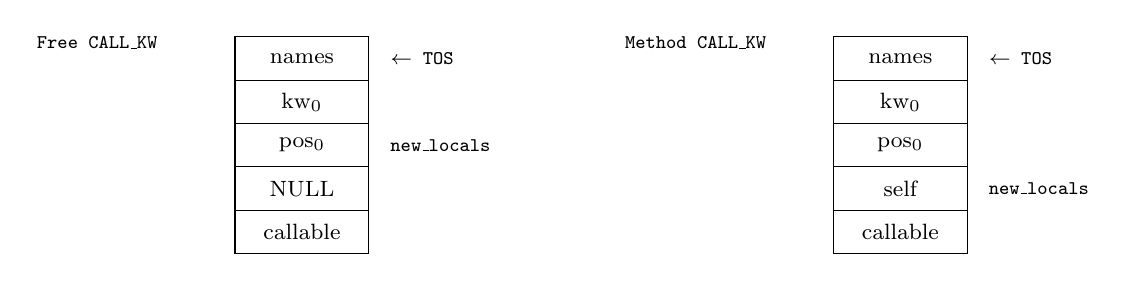
\begin{tikzpicture}[
  font=\footnotesize,
  cell/.style={draw, minimum width=1.7cm, minimum height=0.55cm, align=center},
  lab/.style={font=\scriptsize\ttfamily}
]
  \node[lab] at (-2.6, 2.2) {Free CALL\_KW};
  \foreach \y/\t in {0/names, 1/kw$_0$, 2/pos$_0$, 3/NULL, 4/callable} {
    \node[cell] at (0, 2.0-0.55*\y) {\t};
  }
  \node[lab, right] at (1.0, 2.0) {$\leftarrow$ TOS};
  \node[lab, right] at (1.0, 2.0-0.55*2) {new\_locals};

  \node[lab] at (5.0, 2.2) {Method CALL\_KW};
  \foreach \y/\t in {0/names, 1/kw$_0$, 2/pos$_0$, 3/self, 4/callable} {
    \node[cell] at (7.6, 2.0-0.55*\y) {\t};
  }
  \node[lab, right] at (8.6, 2.0) {$\leftarrow$ TOS};
  \node[lab, right] at (8.6, 2.0-0.55*3) {new\_locals};
\end{tikzpicture}
\caption{Illustrative RF layouts after names are still on stack
(one positional, one keyword).
Method form places \texttt{self} where free calls place NULL; the binder's
kwargs value base is therefore \texttt{argcount} ($= n_{\mathrm{pos}}+1$), not
$n_{\mathrm{pos}}$.}
\label{fig:stack}
\end{figure}

% -----------------------------------------------------------------------------
\section{Code-object metadata consumed by CALL}
% -----------------------------------------------------------------------------

The serialized code object carries a packed metadata integer:

\begin{center}
\begin{tabular}{@{}lp{0.62\textwidth}@{}}
\toprule
Bits & Field \\
\midrule
$[15:0]$ & \texttt{co\_argcount} \\
$[31:16]$ & \texttt{co\_nlocals} \\
$[47:32]$ & \texttt{co\_stacksize} \\
$[63:48]$ & \texttt{co\_kwonlyargcount} \\
$[64]$ & \texttt{CO\_VARARGS} \\
$[65]$ & \texttt{CO\_VARKEYWORDS} \\
$[81:66]$ & \texttt{co\_posonlyargcount} \\
\bottomrule
\end{tabular}
\end{center}

Companion heap fields include \texttt{co\_defaults} (tuple),
\texttt{co\_varnames} (tuple), and \texttt{co\_kwdefaults} (dict).
CPython~3.14 varname order for binding is: positionals, keyword-only, then
\texttt{*args} / \texttt{**kwargs} names.
The binder searches only the formal prefix
$\texttt{argcount}+\texttt{kwonlyargcount}$; vararg names are never keyword
targets---a keyword spelled like \texttt{args} lands in \texttt{**kwargs} when
present.

% -----------------------------------------------------------------------------
\section{The shared binder}
% -----------------------------------------------------------------------------

\subsection{Definition}
The \emph{binder} is the nested micro-sequence under phase~14 (subs~32--55) that
implements CPython argument binding for \texttt{CODE\_OBJECT} callees.
\texttt{CALL}, \texttt{CALL\_KW}, and post-expand \texttt{CALL\_FUNCTION\_EX}
share it.
Phase~6 forces the binder whenever the callee has keyword-only parameters
\emph{or} \texttt{CO\_VARKEYWORDS}, even for a purely positional call---because
an empty \texttt{**kwargs} dict local must still be installed.

\subsection{Pipeline}
Figure~\ref{fig:binder} summarizes the binder pipeline.

\begin{figure}[ht]
\centering
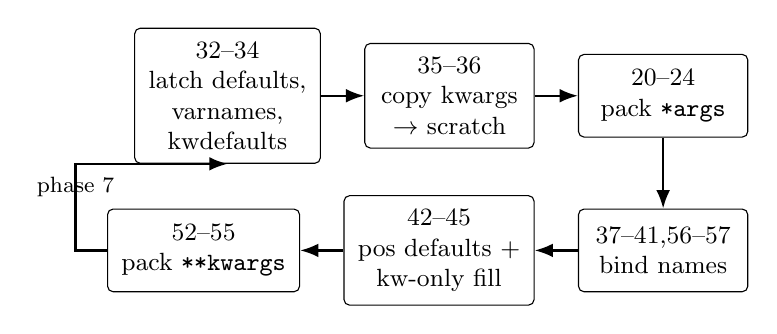
\begin{tikzpicture}[
  font=\small,
  stage/.style={draw, rounded corners=2pt, align=center, inner sep=5pt, minimum height=1.05cm, minimum width=2.15cm},
  arr/.style={-{Latex}, thick}
]
  \node[stage] (a) {32--34\\latch defaults,\\varnames,\\kwdefaults};
  \node[stage, right=0.55cm of a] (b) {35--36\\copy kwargs\\$\to$ scratch};
  \node[stage, right=0.55cm of b] (c) {20--24\\pack \texttt{*args}};
  \node[stage, below=0.9cm of c] (d) {37--41,56--57\\bind names};
  \node[stage, left=0.55cm of d] (e) {42--45\\pos defaults +\\kw-only fill};
  \node[stage, left=0.55cm of e] (f) {52--55\\pack \texttt{**kwargs}};

  \draw[arr] (a) -- (b);
  \draw[arr] (b) -- (c);
  \draw[arr] (c) -- (d);
  \draw[arr] (d) -- (e);
  \draw[arr] (e) -- (f);
  \draw[arr] (f.west) -- ++(-0.4,0) |- node[above, font=\footnotesize, pos=0.25]{phase 7} (a.south);
\end{tikzpicture}
\caption{Shared binder micro-sequence (subs under phase~14).
Calls without keywords skip the scratch copy; callees without
\texttt{CO\_VARARGS}/\texttt{CO\_VARKEYWORDS} skip the corresponding packs.}
\label{fig:binder}
\end{figure}

\subsection{Keyword match rules}
For each caller keyword name $n$:
\begin{enumerate}[leftmargin=*]
  \item Scan formals $k \in [0, \texttt{total\_params})$.
  \item If $n$ matches formal $k$ and $k < \texttt{posonlyargcount}$, treat as
    \emph{unexpected} (positional-only).
  \item If $n$ matches and the slot is already filled $\Rightarrow$
    \texttt{CALL\_FILTER} (duplicate), even when \texttt{**kwargs} exists.
  \item If $n$ matches an unfilled non-posonly formal $\Rightarrow$ write the
    value and mark filled.
  \item If no formal matches $\Rightarrow$ unexpected: record in the leftover
    bitmask when \texttt{CO\_VARKEYWORDS}, else \texttt{CALL\_FILTER}.
\end{enumerate}

\subsection{Variadic packing}
\begin{itemize}[leftmargin=*]
  \item \texttt{*args}: excess positionals are copied into a new tuple installed
    at local index $\texttt{total\_params}$.
  \item \texttt{**kwargs}: leftovers are inserted into a \emph{pre-sized} dict
    (capacity from caller keyword count) so binding never raises
    \texttt{DICT\_GROW}; the handle is installed after positionals, kw-only, and
    \texttt{*args}.
\end{itemize}

% -----------------------------------------------------------------------------
\section{Worked examples}
% -----------------------------------------------------------------------------

\subsection{Positional defaults}
\begin{lstlisting}
def f(a, b=2):
    return a + b
f(1)          # -> 3
\end{lstlisting}
Mode \texttt{POS}, no binder force.
Phase~14 fills $b$ from \texttt{co\_defaults}, bumps
\texttt{call\_argcount} to \texttt{co\_argcount}, then phase~7 clears only
true temporaries.

\subsection{Keyword reorder}
\begin{lstlisting}
def g(a, b):
    return 10*a + b
g(b=4, a=3)   # -> 34
\end{lstlisting}
\texttt{CALL\_KW}: names \texttt{('b','a')}, values below.
Binder matches by \texttt{co\_varnames} and writes locals $[3,4]$.

\subsection{Starred call with empty kwargs}
\begin{lstlisting}
def h(a=0, **k):
    return a + len(k)
h(*(), **{})  # -> 0
\end{lstlisting}
EX expands to a zero-positional call; \texttt{CO\_VARKEYWORDS} forces the
binder; subs~52--55 install an empty dict; defaults supply $a=0$.

\subsection{Positional-only}
\begin{lstlisting}
def p(a, /, b=0, **k):
    return a + 10*b + k.get("a", 0)
p(1, a=2)     # a=1, k={"a": 2}
p_posonly = lambda a, /: a
p_posonly(a=1)  # CALL_FILTER
\end{lstlisting}

\subsection{Bound method + keywords}
\begin{lstlisting}
# o.m is method-form: callable, self, args...
def add(self, a, b=0):
    return a + 10*b
o.m(1, b=2)   # -> 21
\end{lstlisting}
Incoming kwargs sit at $\texttt{locals}[\texttt{argcount}+i]$.
Using $n_{\mathrm{pos}}$ as the source base would read \texttt{self} or a
positional---a latent hole closed when method+kwargs tests landed.

% -----------------------------------------------------------------------------
\section{Important design details}
% -----------------------------------------------------------------------------

\subsection{Latched kwargs scratch bases}
Keyword values are copied from the incoming stack region into a scratch region
\emph{above} real locals so \texttt{*args}/\texttt{**kwargs} packing cannot
clobber them.
The scratch base must be \textbf{latched in binder sub~34}.
A combinational function of \texttt{call\_argcount} is unsafe: the varargs pack
bumps argc, which would move the scratch window and cause later binder reads to
miss parked values (observed as a \texttt{TYPE} trap in
\texttt{*args}+kw-only tests).

Registers:
\begin{itemize}[leftmargin=*]
  \item \texttt{call\_kw\_val\_base\_r} --- source index of incoming kwargs
    (equals effective argc at latch time; includes \texttt{self} for methods).
  \item \texttt{call\_kw\_scratch\_base\_r} --- destination index, at least
    $\texttt{argcount}+n_{\mathrm{kwargs}}$, and at least past
    $\texttt{*args}$/\texttt{**kwargs} local slots when those flags are set.
\end{itemize}

\subsection{Effective argc after default / variadic fill}
Phase~7's UNINIT clear uses $[\texttt{call\_argcount}, \texttt{nlocals})$.
Any value the binder installs into a local---defaults, \texttt{*args},
\texttt{**kwargs}---must be reflected in \texttt{call\_argcount} before phase~7,
or the clear wipes it.
This is the argc==0 defaults-wipe class of bugs; the same discipline applies to
empty \texttt{**kwargs}.

\subsection{Pre-sized \texttt{**kwargs} dict}
Leftover packing sizes the dict for the caller's keyword count up front.
Binding therefore stays on the pycore path without an excore
\texttt{DICT\_GROW} handoff.
The leftover bitmask is 128~bits, matching the binder's 7-bit keyword index
walk.

\subsection{Fatal filters instead of exception objects}
Bad call shapes raise \texttt{PY\_TRAP\_CALL\_FILTER} and halt the simulation /
prototype.
That matches PyCore's current exception story (\texttt{RAISE\_VARARGS} is also
fatal-minimum) and keeps the CALL path free of heap-allocated
\texttt{TypeError} instances.

\subsection{Builtins and kwargs}
\texttt{OBK\_BUILTIN} and raw type objects still reject caller kwargs with
\texttt{CALL\_FILTER}.
Keyword-capable builtins are expected to be ROM firmware \texttt{CODE\_OBJECT}s
(e.g.\ \texttt{print}) so they reuse the same binder.

% -----------------------------------------------------------------------------
\section{Tradeoffs}
% -----------------------------------------------------------------------------

\begin{table}[ht]
\centering
\begin{tabular}{@{}p{0.28\textwidth}p{0.30\textwidth}p{0.30\textwidth}@{}}
\toprule
Choice & Benefit & Cost / alternative \\
\midrule
Shared binder for CALL / CALL\_KW / EX
  & One CPython-shaped semantics path; EX becomes expand-then-bind
  & Larger phase-14 sub-FSM; harder to reason about in isolation \\
\addlinespace
Function $\equiv$ code object
  & Simple image model; defaults on the code handle
  & No per-closure function objects yet; \texttt{MAKE\_FUNCTION} attributes
    limited \\
\addlinespace
Pre-sized \texttt{**kwargs}
  & No grow trap during bind; deterministic cycle bound for $n_{\mathrm{kw}}$
  & Over-allocates when many keywords bind to formals; 128-kw leftover cap \\
\addlinespace
Latch scratch bases
  & Correct under argc mutation from \texttt{*args}
  & Extra registers; easy to regress if a new path recomputes combinationally \\
\addlinespace
Fatal \texttt{CALL\_FILTER}
  & Small RTL; clear differential tests against host \texttt{TypeError}
  & Not source-compatible with \texttt{try}/\texttt{except TypeError} yet \\
\addlinespace
Builtin kwargs via firmware
  & Avoids per-\texttt{BI\_*} keyword tables in RTL
  & Builtin fast path and firmware path must stay behaviorally aligned \\
\bottomrule
\end{tabular}
\caption{Design tradeoffs in the CALL / binder implementation.}
\label{tab:tradeoffs}
\end{table}

\paragraph{Cycle cost vs.\ semantic fidelity.}
PyCore deliberately spends cycles on name compares and dict probes rather than
approximating ``positional only forever.''
The research claim is that a bytecode-native CPU can host real CPython call
shapes; the binder is where that claim is won or lost.

\paragraph{Testing strategy.}
Differential image tests (\texttt{run\_image\_test.py}) execute the same source
on CPython~3.14 for a golden tag/value, then in Verilator.
Trap tests encode expected \texttt{CALL\_FILTER} without host execution.
The suite \texttt{pycore-img-call-all} is the regression gate for this FSM.

% -----------------------------------------------------------------------------
\section{Limits and non-goals}
% -----------------------------------------------------------------------------

\begin{itemize}[leftmargin=*]
  \item No rich exception objects or exception handlers on the CALL path.
  \item Leftover-keyword bitmask width 128 (binder index width).
  \item Non-string / contaminated EX kwargs keys trap during bind.
  \item Closures / cell variables are outside the interim function model.
  \item Full LEGB for nested scopes remains a separate initiative.
\end{itemize}

% -----------------------------------------------------------------------------
\section{Reference map}
% -----------------------------------------------------------------------------

\begin{center}
\begin{tabular}{@{}lp{0.62\textwidth}@{}}
\toprule
Artifact & Role \\
\midrule
\texttt{pycore/rtl/pycore\_call\_fsm.svh} & Phase/binder implementation \\
\texttt{pycore/rtl/pycore\_core.sv} & \texttt{S\_CALL} state, mode/phase locals, scratch latch wires \\
\texttt{pycore/rtl/pycore\_defs.svh} & Metadata bitfields, trap codes, opcodes \\
\texttt{pycore/tools/encoding.py} & Metadata pack/unpack \\
\texttt{planning/implemented/co\_varkeywords\_call\_parity.md} & Recent parity delta + test matrix \\
\texttt{pycore/docs/bytecode\_support.md} & Opcode support matrix \\
\texttt{Makefile} \texttt{pycore-img-call-all} & Hardware regression aggregate \\
\bottomrule
\end{tabular}
\end{center}

% -----------------------------------------------------------------------------
\section{Conclusion}
% -----------------------------------------------------------------------------

The CALL FSM is the semantic gate between CPython's calling convention and
PyCore's frame/locals machine.
Its important idea is not a clever opcode encoding but a \emph{shared binder}
that makes \texttt{CALL}, \texttt{CALL\_KW}, and \texttt{CALL\_FUNCTION\_EX}
converge on one CPython-faithful binding procedure, with explicit handling for
defaults, positional-only parameters, and variadic locals.
With that path complete for user code objects, subsequent paper systems---ROM
firmware builtins, richer objects, and language-level features that assume
ordinary calls---can build on a stable foundation.

\end{document}
